%!TEX program = xelatex
%!TEX encoding = UTF-8 Unicode
\documentclass{beamer}
\usepackage[english,russian]{babel}

\usetheme{Execushares}
\usepackage{setspace}
\usepackage{color}
\usepackage{inconsolata}
\setmonofont[BoldFont=*,BoldFeatures={FakeBold=1.4},
  ItalicFont=*,ItalicFeatures={FakeSlant=0.2},
  BoldItalicFont=*,BoldItalicFeatures={FakeBold=1.4,FakeSlant=0.2}
  ]{Consolas}
\usepackage{listings}

\definecolor{listinggray}{gray}{0.9}
\definecolor{lbcolor}{rgb}{0.9,0.9,0.9}

\lstset{
  backgroundcolor=\color{lbcolor},
  tabsize=4,
  language=C++,
  captionpos=b,
  frame=lines,
  numbers=left,
  numberstyle=\tiny,
  numbersep=5pt,
  breaklines=true,
  showstringspaces=false,
  basicstyle=\ttfamily\footnotesize,
  keywordstyle=\color[rgb]{0,0,1},
  stringstyle=\color{red}
}

% \usepackage{enumitem}
% \usepackage{amsfonts}

\title{Контролируемое исполнение программ в~многозадачном окружении}
\author{Защищается: студент группы Б8403А \\ Ротанов Денис Владимирович \\ Руководитель: старший преподаватель \\ Кленин Александр Сергеевич}

\institute{Дальневосточный Федеральный университет, 2015г.}

\setcounter{showSlideNumbers}{1}

\begin{document}

\setcounter{showProgressBar}{0}
\setcounter{showSlideNumbers}{0}

\frame{\titlepage}

\setcounter{framenumber}{0}
\setcounter{showProgressBar}{1}
\setcounter{showSlideNumbers}{1}

\section{Предметная область}

\begin{frame}
  \frametitle{Спортивное программирование}
  \begin{enumerate}
    \item Олимпиады школьников по программированию
    \item ACM ICPC (международная студенческая олимпиада)
    \item Соревнования искуственного интеллекта
  \end{enumerate}
\end{frame}

% \begin{frame}[fragile]
% \begin{large}
%     Contexte : \newline \pause
% \end{large}

% \begin{itemize}
%     \item Avertir Drupal
% \end{itemize}
% \begin{lstlisting}
% #include<stdio.h>
% #include<iostream>
% // A comment
% int main(void)
% {
%   printf("Hello World\n");
%   return 0;
% }
% \end{lstlisting}
% \end{frame}

% \begin{frame}
%   \frametitle{Контролируемое исполнение}

%   Sandboxing
%   \begin{itemize}
%     \item Безопасность
%     \item Контроль потребления ресурсов
%   \end{itemize}

% \end{frame}

% \begin{frame}
%   \frametitle{Приложения Sandboxing'a}
%   \begin{itemize}
%     \item Online IDE
%     \item Advanced pastebins
%     \item Continuous integration
%     \item Aнтивирусы
%     \item Тестирующие системы
%   \end{itemize}
% \end{frame}

\begin{frame}
  \frametitle{Соревнования ИИ}
  \begin{itemize}
  \item виртуальная среда
  \item интеллектуальные агенты
  \item многозадачность (в смысле процессов ОС)
  \item управляющая программа
  \item нормальная программа
  \end{itemize}
\end{frame}

\begin{frame}
  \frametitle{Соревнования ИИ - Примеры [1]}
  \begin{figure}[htb]
  \centering
  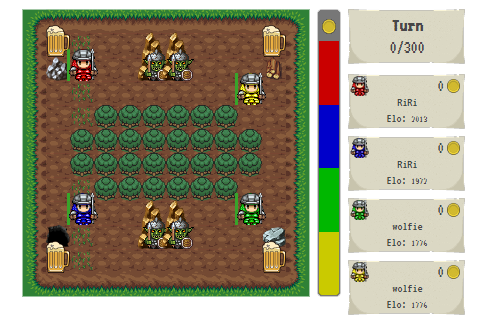
\includegraphics[height=6cm,keepaspectratio]{./img/vindinium.png}
  \caption{Vindinium}
  \end{figure}
\end{frame}

\begin{frame}
  \frametitle{Соревнования ИИ - Примеры [2]}
  \begin{figure}[htb]
  \centering
  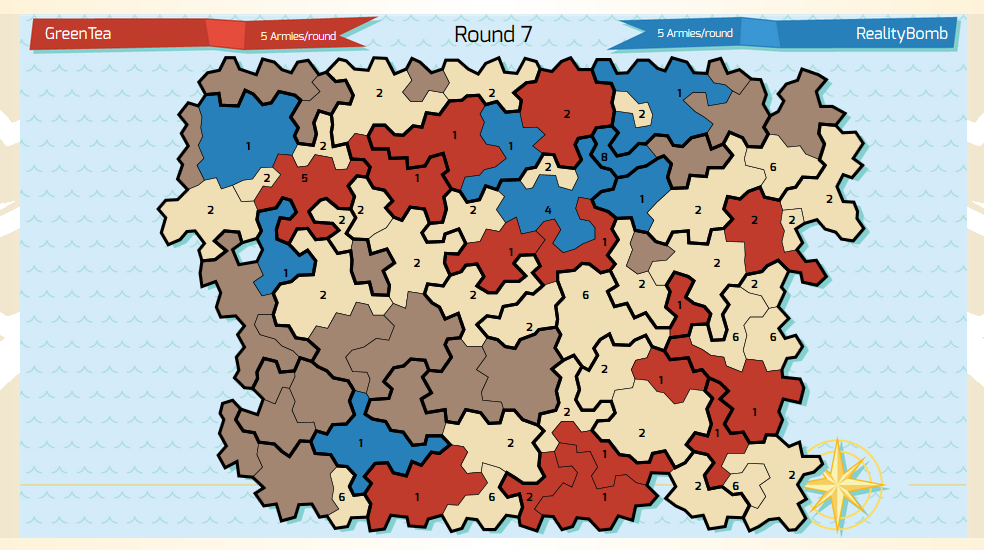
\includegraphics[height=6cm,keepaspectratio]{./img/warlight.png}
  \caption{theaigames - Warlight 2 Challenge}
  \end{figure}
\end{frame}

\begin{frame}
  \frametitle{Соревнования ИИ - Примеры [3]}
  \begin{figure}[htb]
  \centering
  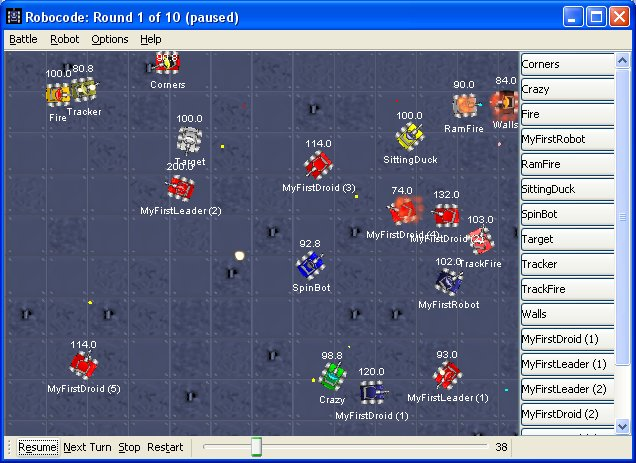
\includegraphics[height=6cm,keepaspectratio]{./img/robocode.jpg}
  \caption{Robocode}
  \end{figure}
\end{frame}

\begin{frame}
  \frametitle{Соревнования ИИ - Примеры [4]}
  \begin{figure}[htb]
  \centering
  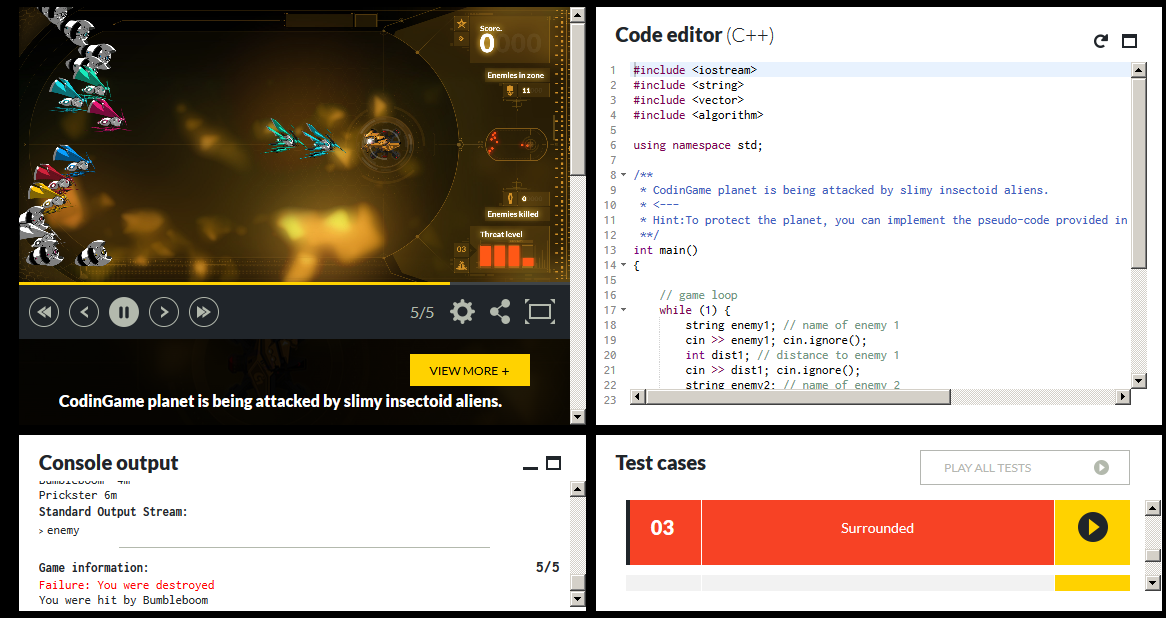
\includegraphics[height=6cm,keepaspectratio]{./img/codingame.png}
  \caption{Codingame}
  \end{figure}
\end{frame}

\begin{frame}
  \frametitle{CATS - автоматизация~соревнований}
  \begin{figure}[htb]
  \centering
  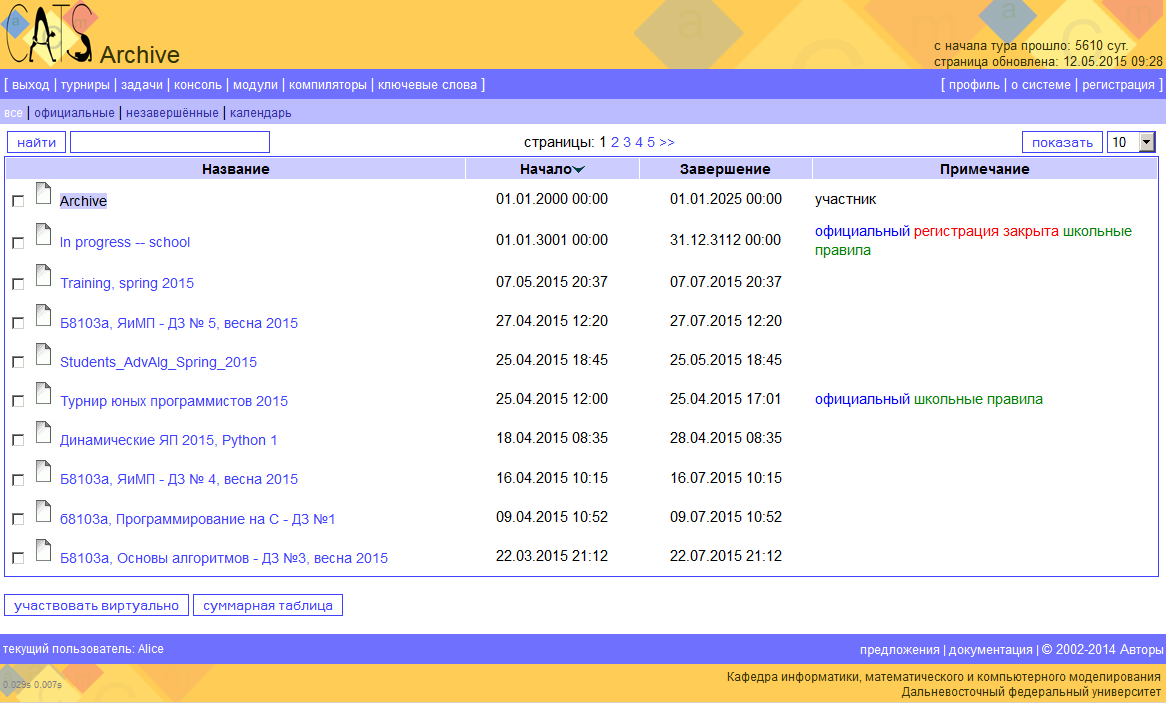
\includegraphics[width=8cm,keepaspectratio]{./img/cats_screenshot.png}
  \end{figure}
  CATS - система автоматической проверки решений задач по~программированию
\end{frame}

\begin{frame}
  \frametitle{Компоненты CATS}
  \begin{figure}[htb]
  \centering
  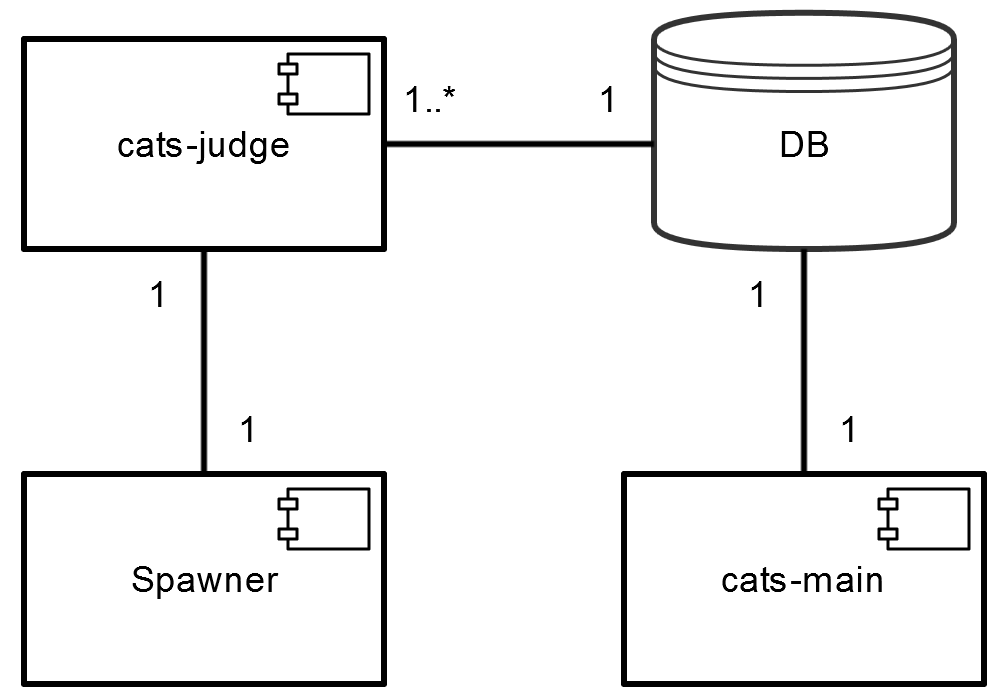
\includegraphics[width=8cm,keepaspectratio]{./img/cats.png}
  \end{figure}
\end{frame}

\begin{frame}
  \frametitle{Типы задач}
  \begin{itemize}
    \item Стандартные
    \item Интерактивные
    \item Многоагентные
  \end{itemize}
\end{frame}

\begin{frame}
  \frametitle{Стандартные задачи}
  \begin{figure}[htb]
  \centering
  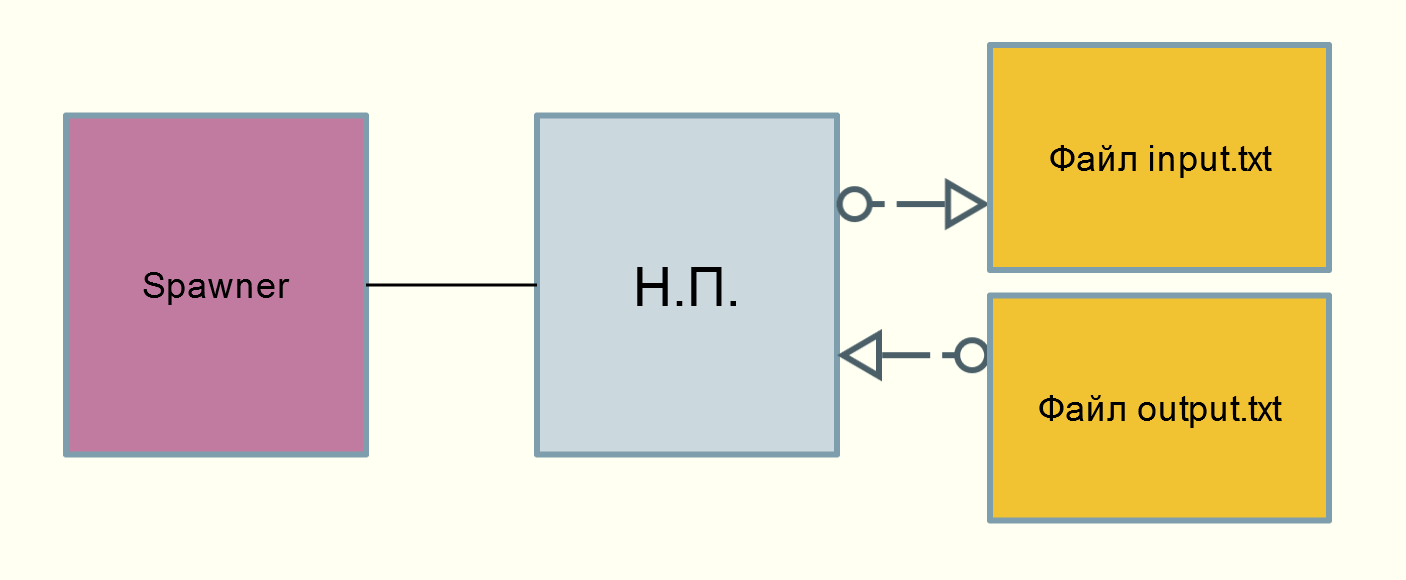
\includegraphics[width=\textwidth,keepaspectratio]{./img/normal_data_flow.png}
  \end{figure}
\end{frame}

\begin{frame}
  \frametitle{Интерактивные задачи}
  \begin{figure}[htb]
  \centering
  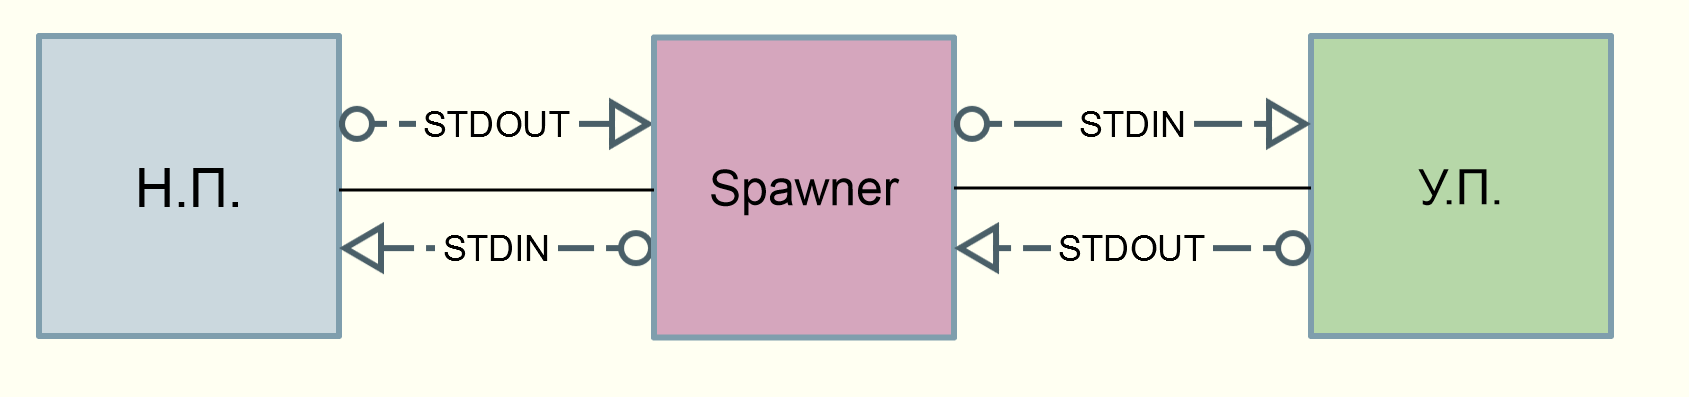
\includegraphics[width=\textwidth,keepaspectratio]{./img/interactive_data_flow.png}
  \end{figure}
\end{frame}

\begin{frame}
  \frametitle{Многоагентные задачи}
  \begin{figure}[htb]
  \centering
  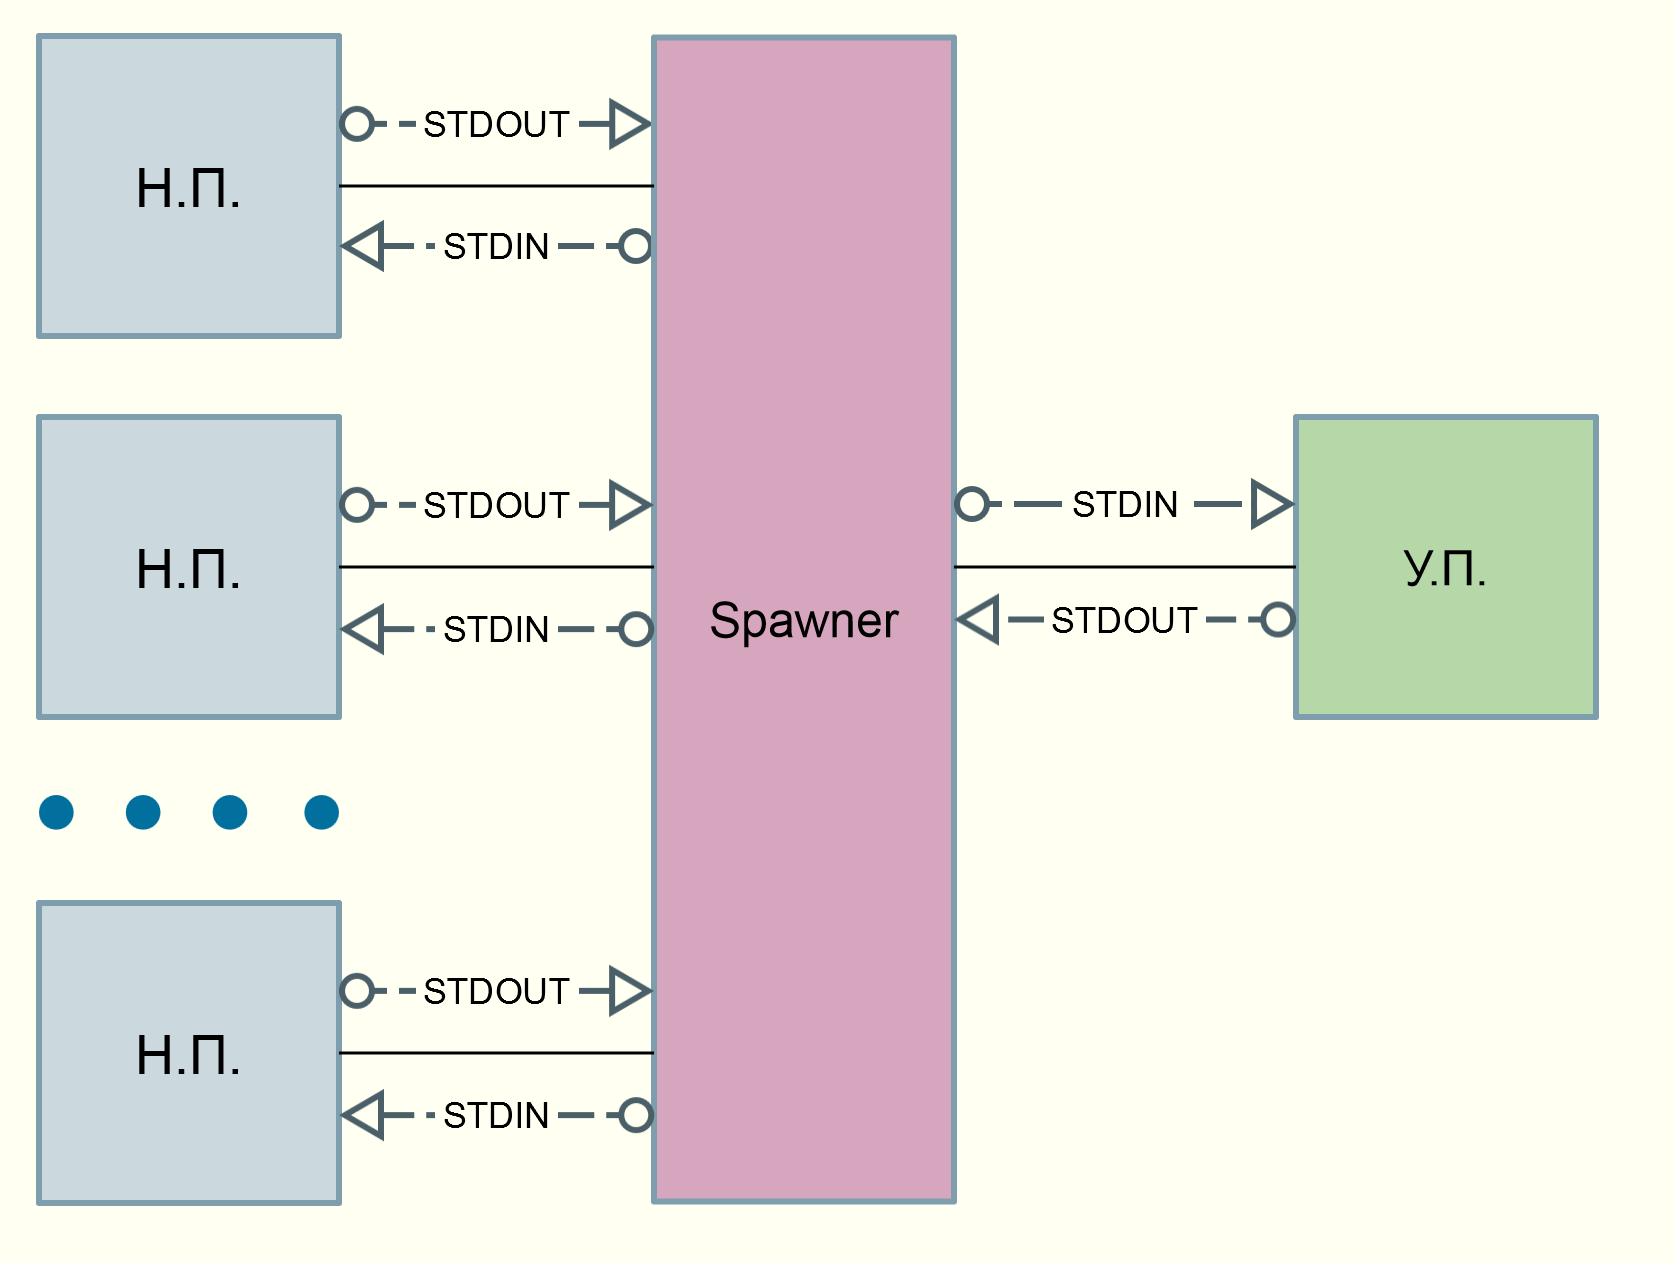
\includegraphics[height=6cm,keepaspectratio]{./img/multiagent_data_flow.png}
  \end{figure}
\end{frame}

\section{Цель работы}

\begin{frame}
  \frametitle{Цель работы}
  Расширение класса задач, поддерживаемых CATS:
  \begin{itemize}
  \item интерактивные задачи
  \item многоагентные задачи
  \end{itemize}
\end{frame}

\begin{frame}
  \frametitle{Существующие решения}
  \begin{itemize}
  \item аналоги CATS
    \begin{itemize}
    \item[\checkmark] интерактивные задачи
    \item[$\times$] многоагентные задачи
    \end{itemize}
  \item системы соревнований ИИ
    \begin{itemize}
    \item узкоспециализированы (1 задача)
    \end{itemize}
  \item средства контролируемого исполнения
    \begin{itemize}
    \item[$\times$] связь стандартных потоков
    \item[$\times$] делегирование управления
    \end{itemize}
  \end{itemize}
\end{frame}

\section{Основные проектные решения}

\begin{frame}[fragile]
  \frametitle{Потоки ввода-вывода}

\begin{lstlisting}
#include <cstdio>
int main()
{
  // STDOUT:
  printf("Hello World\n");

  // STDIN:
  int n = -1;
  scanf("%d", &n);
}
\end{lstlisting}
\end{frame}

% \begin{frame}
%   \frametitle{К.И. и Многозадачность}
%   \begin{enumerate}
%     \item запрещающие многозадачность
%     \item индифферентные к многозадачности
%     \item поддерживающие многозадачность
%   \end{enumerate}
% \end{frame}

% \begin{frame}
%   \frametitle{Интерактивные задачи}
%   Классы задач:
%   \begin{itemize}
%     \item online-алгоритмы
%     \item игровые задачи
%     \item программы управления
%   \end{itemize}
% \end{frame}

% \section{Существующие решения}
% \begin{frame}
%   \frametitle{Существующие решения}
%   Системы автоматической проверки задач:
%   \begin{itemize}
%     \item CATS
%     \item ejudge
%     \item PCMS2
%     \item Contester
%     \item PC$^2$
%     \item DOMjudge
%     \item dudge
%   \end{itemize}
%   % Большинство данных систем поддерживают интерактивные задачи. CATS --- теперь тоже.
%   % Ни одно из рассмотренных решений не предоставляет средств для проведения AI-турниров.
% \end{frame}

\section{Проект и реализация}

% \begin{frame}
%   \frametitle{Функциональные требования}
%   \begin{itemize}
%     \item пёс
%     \item кот
%   \end{itemize}
% \end{frame}
% \begin{frame}
%   \frametitle{Интерактивные Задачи}
%   \begin{itemize}
%     \item Понятие run\_method добавлено в DB для таблицы Problems, в парсер формата задачи, cats-judge обучен run\_method (нужные строки запуска Spawner добавлены в конфиг)
%     \item Успешный вызов в интерактивном режиме так же обеспечен для задач, интеракторы которых реализованы на интерпретируемых языках, таких как Java; за счёт абстрагирования от строки указывающей на программу-интерактор в строке запуска Spawner.
%     \item Продемонстировано, что указание в настройках задачи run\_method=interactive, а так же предъявления некоторых требований к самой задаче достаточно для интерактивных задач на примере двух задач. (интерактивное сложение, NEERC gomoku)
%   \end{itemize}
% \end{frame}

% \begin{frame}
%   \frametitle{controller - normal}
%   \begin{itemize}
%     \item связать controller и normal
%       \begin{enumerate}
%         \item controller запускает spawner для каждого normal
%         \item Только std pipes, префиксный протокол
%         \item named pipes
%         \item через файлы
%       \end{enumerate}
%     \item Сообщать интерактору количество клиентов
%     \item controller управляет spawner
%   \end{itemize}
% \end{frame}

\begin{frame}[fragile]
  \frametitle{Реализация интерактивных задач}
Настройки задачи:
\begin{lstlisting}
<Problem title="online addition" lang="ru" tlimit="1"
  mlimit="256" inputFile="*STDIN" outputFile="*STDOUT">

  <Run method="interactive"/>
...
</Problem>
\end{lstlisting}
Настройки cats-judge:
\begin{lstlisting}
<define name="#run_interactive" value="#spawner
  --separator=// -hr=1 --out=nul -wl=30 -tl=%time_limit
  -ml=%memory_limit -y=1 --// -sr=report.txt
  --in=*1.stdout --out=*1.stdin %interactor_name
  --// %deadline -sr= "/>
\end{lstlisting}
\end{frame}

\begin{frame}
  \frametitle{Интерактивные задачи}
  \begin{figure}[htb]
  \centering
  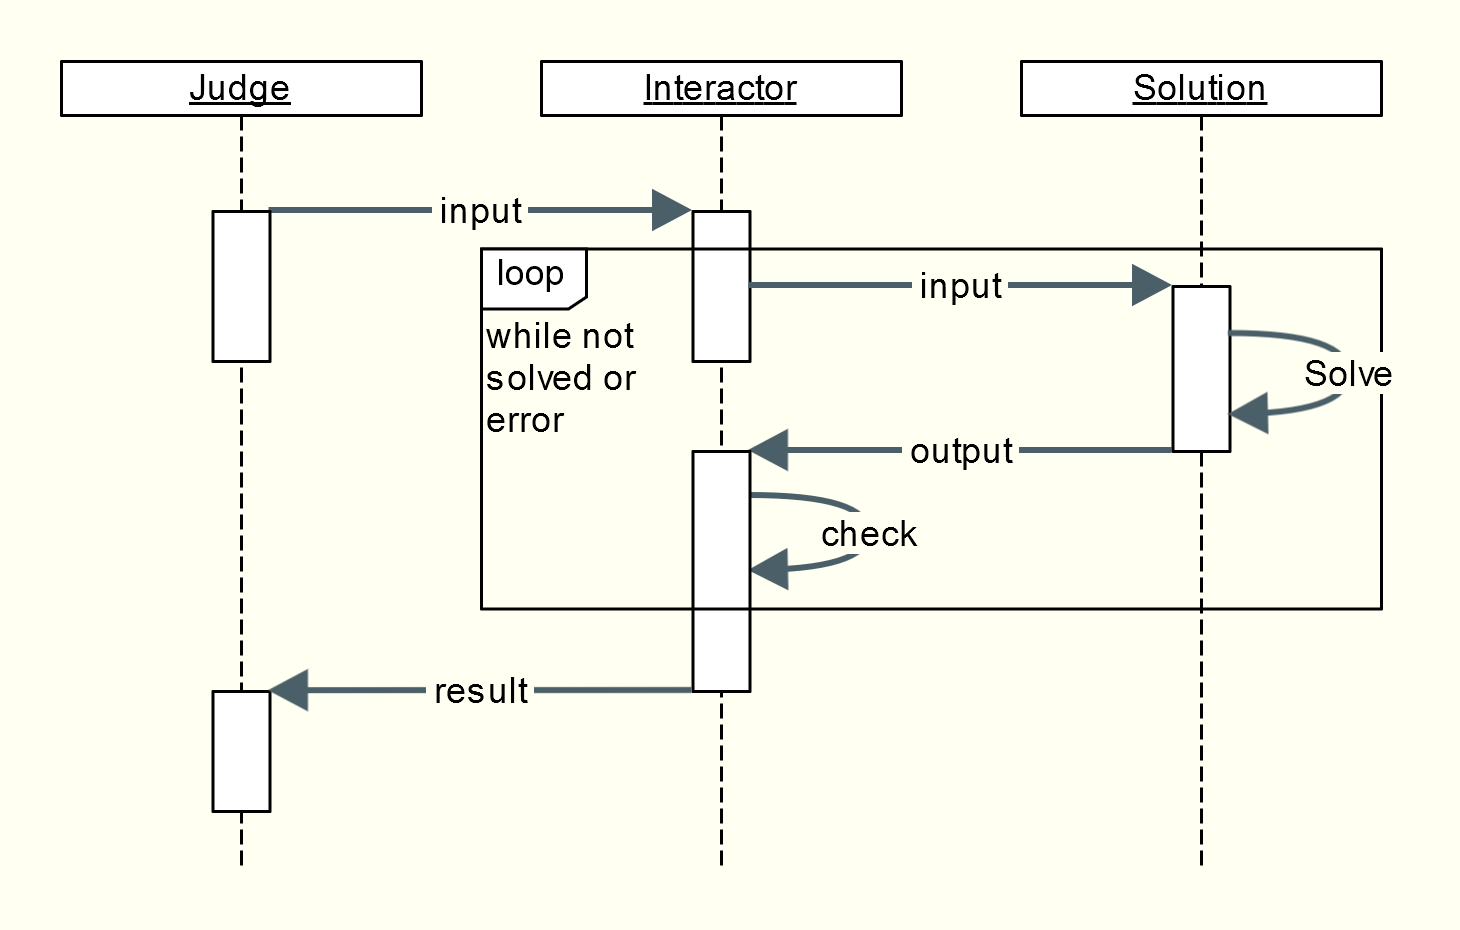
\includegraphics[height=6cm,keepaspectratio]{./img/interactive_problem.png}
  \end{figure}
\end{frame}

\begin{frame}
  \frametitle{Реализация многоагентных задач}
  \begin{itemize}
  \item каждый процесс - два потока
  \item n процессов
  \item связь одного процесса со многими
  \item мультиплексирование потоков
  \item протокол
  \end{itemize}
\end{frame}

\begin{frame}[fragile]
  \frametitle{Протокол}
  \begin{itemize}
  \item гарантия атомарности сообщений
  \item {
  У.П.: отослать сообщение Н.П.[i]
\begin{lstlisting}
printf("i#<message>\n");
fflush(stdout);
\end{lstlisting}
}
  \item { У.П.: завершить Н.П.[i]
\begin{lstlisting}
printf("iS#\n");
fflush(stdout);
\end{lstlisting}
}
  \item { У.П.: ожидать сообщения от Н.П.[i]
\begin{lstlisting}
printf("iW#\n");
fflush(stdout);
\end{lstlisting}
}
  \item Spawner должен помечать сообщения от Н.П.
  \end{itemize}
\end{frame}

\begin{frame}[fragile]
  \frametitle{Командная~строка~запуска~Spawner}

\begin{lstlisting}
sp.exe -tl=1 -d=2 --separator=//
--// -tl=5 -d=5 --controller controller.exe 3
--// --in=*0.stdout --out=*0.stdin normal-1.exe
--// --in=*0.stdout --out=*0.stdin normal-2.exe
--// --in=*0.stdout --out=*0.stdin normal-3.exe
\end{lstlisting}
\end{frame}

% \begin{frame}
%   \frametitle{Стандартные задачи}
%   \begin{figure}[htb]
%   \centering
%   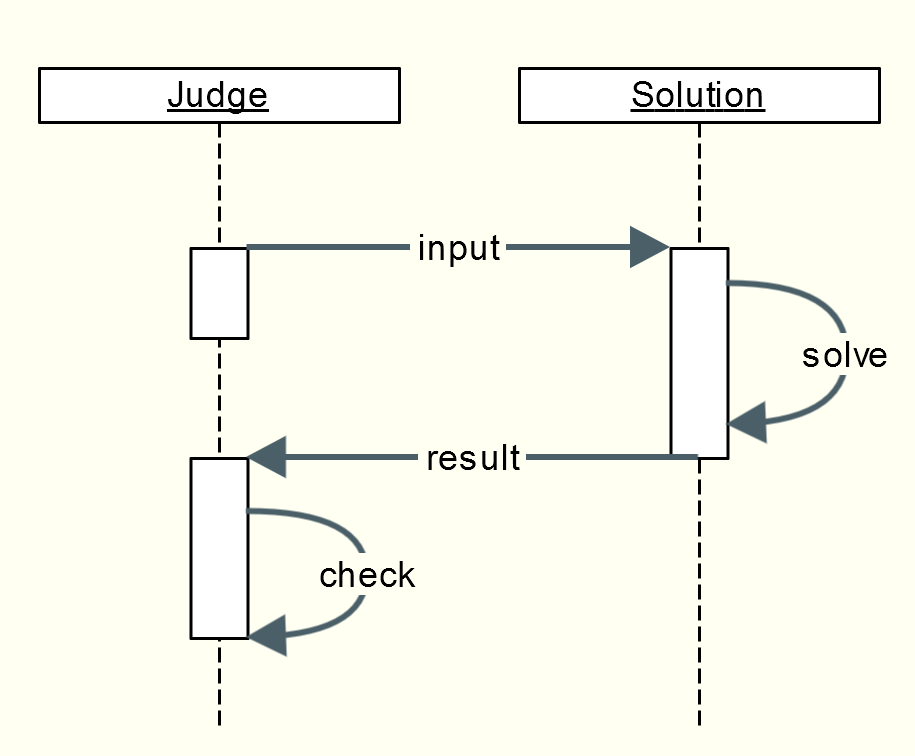
\includegraphics[height=6cm,keepaspectratio]{./img/normal_problem.png}
%   \end{figure}
% \end{frame}

\begin{frame}
  \frametitle{Многоагентные задачи}
  \begin{figure}[htb]
  \centering
  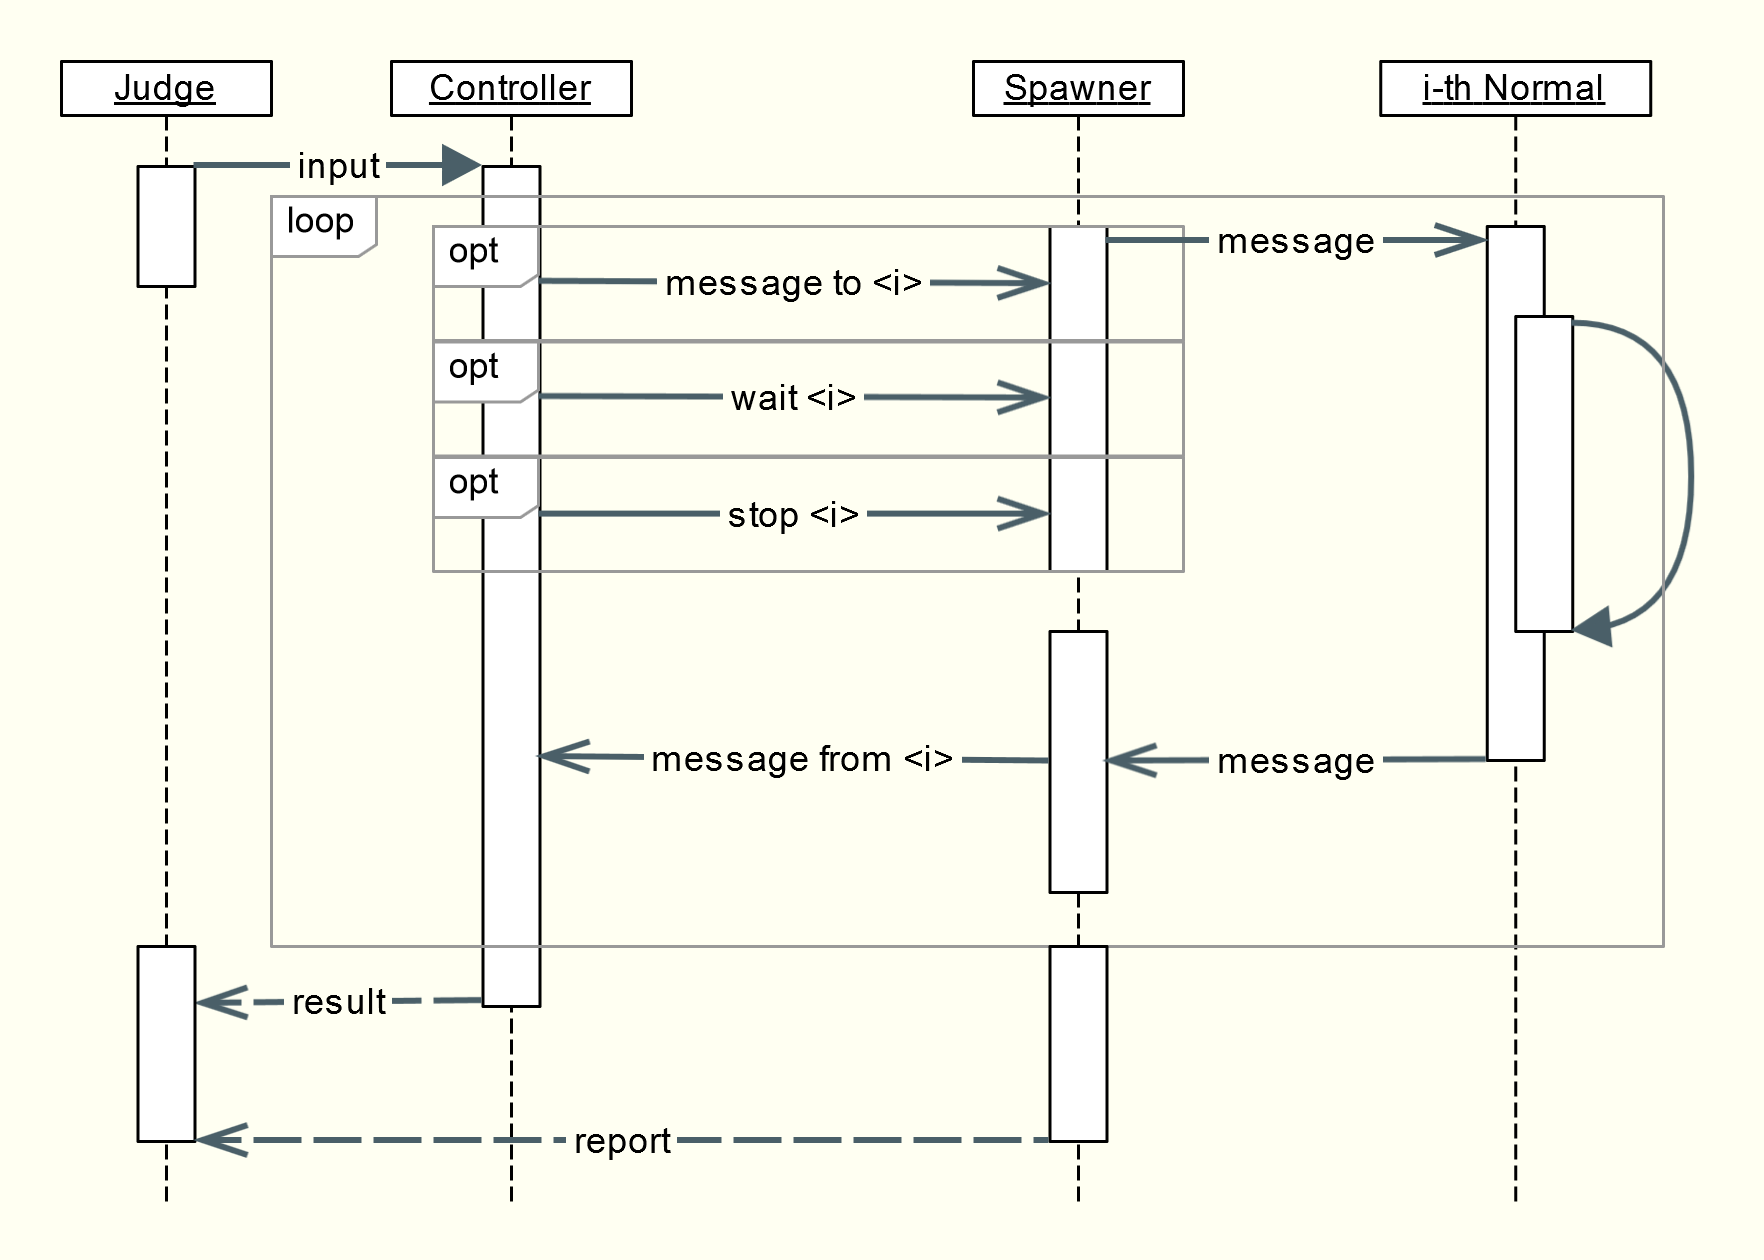
\includegraphics[height=6cm,keepaspectratio]{./img/ai_contest_problem.png}
  \end{figure}
\end{frame}

\begin{frame}
  \frametitle{Связь ввода-вывода процессов}
  \begin{figure}[htb]
  \centering
  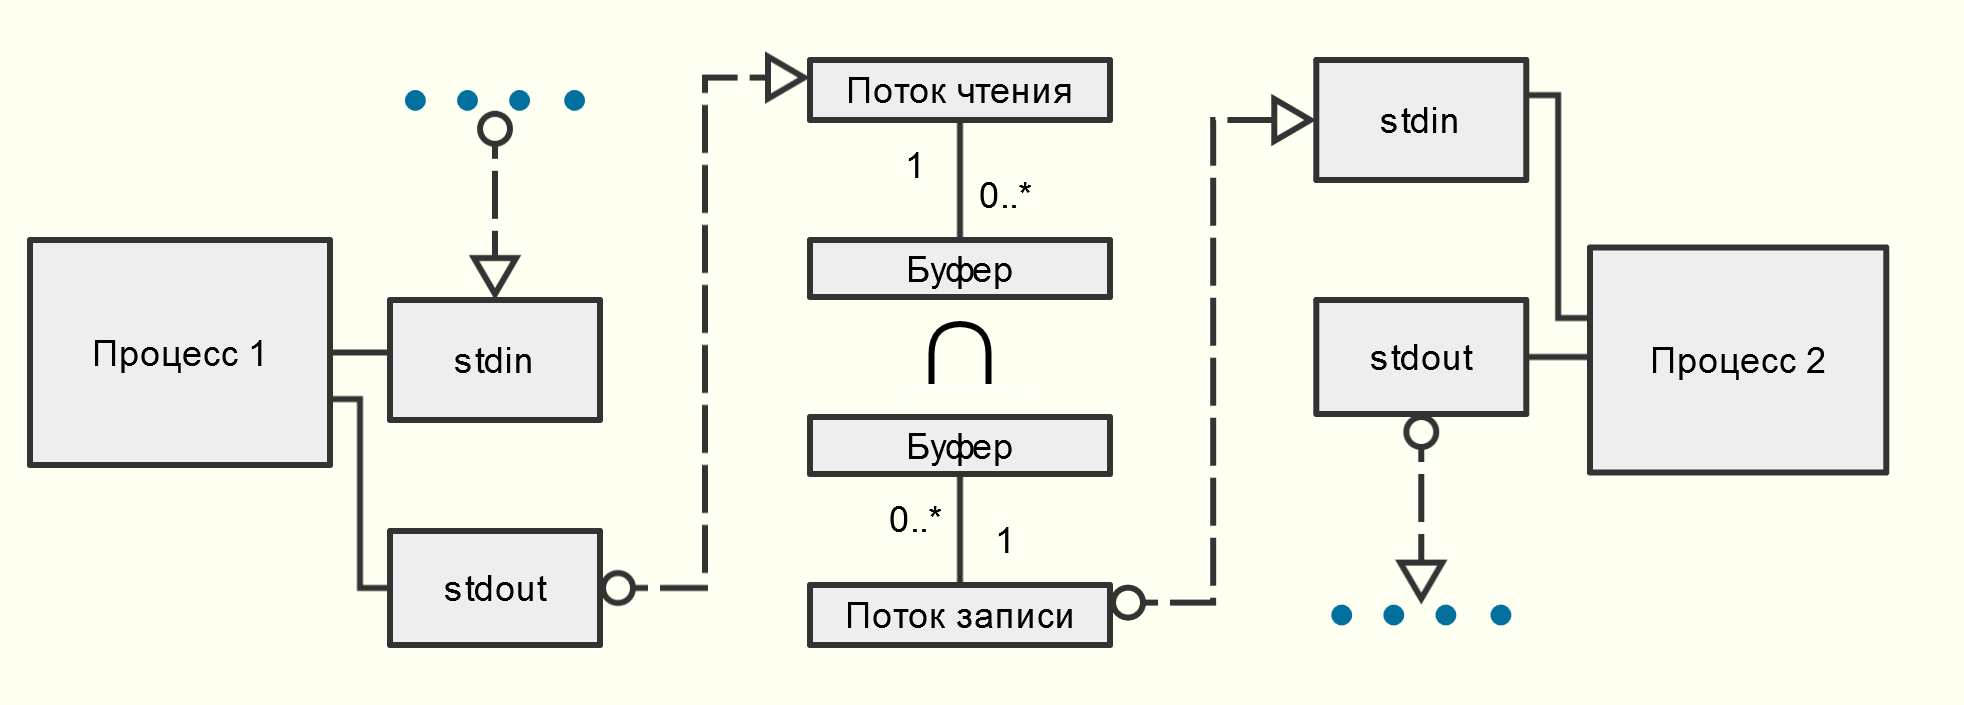
\includegraphics[width=\textwidth,keepaspectratio]{./img/data_flow.png}
  \label{ai_contest_problem}
  \end{figure}
\end{frame}

\begin{frame}
  \frametitle{Тестирование}
  \begin{itemize}
  \item примеры интерактивных задач
  \item примеры многоагентных задач
  \item многократный запуск многоагентных задач
  \item сборка проекта различными компиляторами C++
  \end{itemize}
\end{frame}

\section{Заключение}
\begin{frame}
  \frametitle{Заключение}
  \begin{itemize}
    \item реализована поддержка интерактивных задач в CATS
    \item разработан протокол обмена данными для задач
    \item модуль Spawner:
    \begin{itemize}
    \item реализована поддержка протокола
    \item произведён рефакторинг
    \item исправлены ошибки
    \end{itemize}
    \item ~4500 строк кода
    \item 61 коммит в репозитории проектов CATS
  \end{itemize}
\end{frame}

\end{document}
